\documentclass[border=10pt]{standalone}
\usepackage{tikz}
\usepackage{tikz}
\usepackage{circuitikz}
\usetikzlibrary{arrows,positioning,shapes.geometric}
\begin{document}
\begin{normalsize}
 \tikzset{every picture/.style={line width=0.75pt}} %set default line width to 0.75pt        

\tikzset{every picture/.style={line width=0.75pt}} %set default line width to 0.75pt        

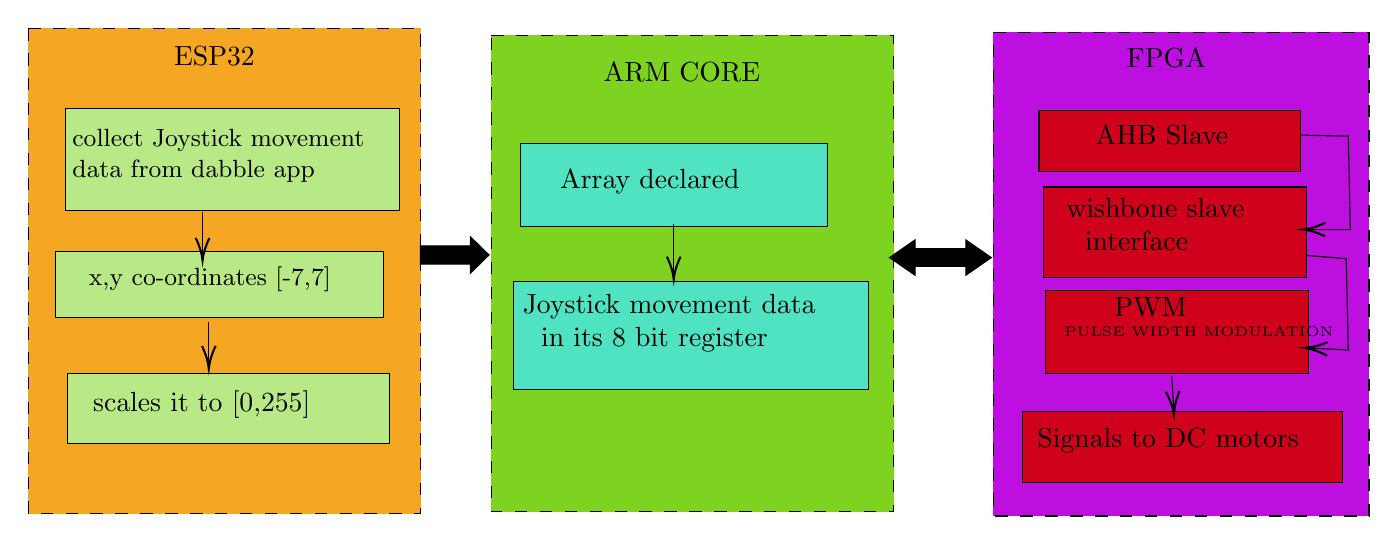
\begin{tikzpicture}[x=0.75pt,y=0.75pt,yscale=-1,xscale=1]
%uncomment if require: \path (0,488); %set diagram left start at 0, and has height of 488

%Shape: Rectangle [id:dp9155852856174811] 
\draw  [fill={rgb, 255:red, 245; green, 166; blue, 35 }  ,fill opacity=1 ][dash pattern={on 4.5pt off 4.5pt}] (8,0.5) -- (197,0.5) -- (197,234.5) -- (8,234.5) -- cycle ;
%Shape: Rectangle [id:dp3128926879300873] 
\draw  [fill={rgb, 255:red, 126; green, 211; blue, 33 }  ,fill opacity=1 ][dash pattern={on 4.5pt off 4.5pt}] (231,4) -- (425,4) -- (425,233.5) -- (231,233.5) -- cycle ;
%Shape: Rectangle [id:dp9408237411863776] 
\draw  [fill={rgb, 255:red, 189; green, 16; blue, 224 }  ,fill opacity=1 ][dash pattern={on 4.5pt off 4.5pt}] (473,2.5) -- (654,2.5) -- (654,235.5) -- (473,235.5) -- cycle ;
%Shape: Rectangle [id:dp18933840597790896] 
\draw  [fill={rgb, 255:red, 184; green, 233; blue, 134 }  ,fill opacity=1 ] (26,39) -- (187,39) -- (187,88.5) -- (26,88.5) -- cycle ;
%Shape: Rectangle [id:dp5329846385294584] 
\draw  [fill={rgb, 255:red, 184; green, 233; blue, 134 }  ,fill opacity=1 ] (21,108.25) -- (179,108.25) -- (179,139.75) -- (21,139.75) -- cycle ;
%Shape: Rectangle [id:dp9019413502494702] 
\draw  [fill={rgb, 255:red, 184; green, 233; blue, 134 }  ,fill opacity=1 ] (27,167) -- (182,167) -- (182,200.5) -- (27,200.5) -- cycle ;
%Straight Lines [id:da873437358806408] 
\draw    (92,89) -- (92,110.5) ;
\draw [shift={(92,112.5)}, rotate = 270] [color={rgb, 255:red, 0; green, 0; blue, 0 }  ][line width=0.75]    (10.93,-3.29) .. controls (6.95,-1.4) and (3.31,-0.3) .. (0,0) .. controls (3.31,0.3) and (6.95,1.4) .. (10.93,3.29)   ;
%Straight Lines [id:da7020327619014652] 
\draw    (95,142) -- (95,162.5) ;
\draw [shift={(95,164.5)}, rotate = 270] [color={rgb, 255:red, 0; green, 0; blue, 0 }  ][line width=0.75]    (10.93,-3.29) .. controls (6.95,-1.4) and (3.31,-0.3) .. (0,0) .. controls (3.31,0.3) and (6.95,1.4) .. (10.93,3.29)   ;
%Shape: Rectangle [id:dp6620929943188993] 
\draw  [fill={rgb, 255:red, 80; green, 227; blue, 194 }  ,fill opacity=1 ] (245,56) -- (393,56) -- (393,96) -- (245,96) -- cycle ;
%Shape: Rectangle [id:dp43628427459438646] 
\draw  [fill={rgb, 255:red, 80; green, 227; blue, 194 }  ,fill opacity=1 ] (242,122.5) -- (413,122.5) -- (413,174.5) -- (242,174.5) -- cycle ;
%Shape: Rectangle [id:dp36235300847534235] 
\draw  [fill={rgb, 255:red, 208; green, 2; blue, 27 }  ,fill opacity=1 ] (495,40) -- (621,40) -- (621,69.5) -- (495,69.5) -- cycle ;
%Shape: Rectangle [id:dp08164777649415955] 
\draw  [fill={rgb, 255:red, 208; green, 2; blue, 27 }  ,fill opacity=1 ] (497,77) -- (624,77) -- (624,120.5) -- (497,120.5) -- cycle ;
%Shape: Rectangle [id:dp9341829336392721] 
\draw  [fill={rgb, 255:red, 208; green, 2; blue, 27 }  ,fill opacity=1 ] (498,127) -- (625,127) -- (625,167) -- (498,167) -- cycle ;
%Left Right Arrow [id:dp06576702254503808] 
\draw  [fill={rgb, 255:red, 0; green, 0; blue, 0 }  ,fill opacity=1 ] (423,111) -- (435.25,102.5) -- (435.25,106.75) -- (459.75,106.75) -- (459.75,102.5) -- (472,111) -- (459.75,119.5) -- (459.75,115.25) -- (435.25,115.25) -- (435.25,119.5) -- cycle ;
%Right Arrow [id:dp9377840575153946] 
\draw  [fill={rgb, 255:red, 0; green, 0; blue, 0 }  ,fill opacity=1 ] (197,105.38) -- (221.04,105.38) -- (221.04,101) -- (230,109.75) -- (221.04,118.5) -- (221.04,114.13) -- (197,114.13) -- cycle ;
%Shape: Rectangle [id:dp3116985902185355] 
\draw  [fill={rgb, 255:red, 208; green, 2; blue, 27 }  ,fill opacity=1 ] (487,185) -- (641,185) -- (641,219.5) -- (487,219.5) -- cycle ;
%Straight Lines [id:da7623767790171208] 
\draw    (319,95) -- (319,119.5) ;
\draw [shift={(319,121.5)}, rotate = 270] [color={rgb, 255:red, 0; green, 0; blue, 0 }  ][line width=0.75]    (10.93,-3.29) .. controls (6.95,-1.4) and (3.31,-0.3) .. (0,0) .. controls (3.31,0.3) and (6.95,1.4) .. (10.93,3.29)   ;
%Straight Lines [id:da5140538118293165] 
\draw    (621,52) -- (644,52.5) -- (645,97.5) -- (624,97.5) ;
\draw [shift={(622,97.5)}, rotate = 360] [color={rgb, 255:red, 0; green, 0; blue, 0 }  ][line width=0.75]    (10.93,-3.29) .. controls (6.95,-1.4) and (3.31,-0.3) .. (0,0) .. controls (3.31,0.3) and (6.95,1.4) .. (10.93,3.29)   ;
%Straight Lines [id:da8380438252502311] 
\draw    (624,110) -- (643,111.5) -- (644,155.5) -- (625,154.6) ;
\draw [shift={(623,154.5)}, rotate = 2.73] [color={rgb, 255:red, 0; green, 0; blue, 0 }  ][line width=0.75]    (10.93,-3.29) .. controls (6.95,-1.4) and (3.31,-0.3) .. (0,0) .. controls (3.31,0.3) and (6.95,1.4) .. (10.93,3.29)   ;
%Straight Lines [id:da12456714228967636] 
\draw    (559,168) -- (559.89,184.5) ;
\draw [shift={(560,186.5)}, rotate = 266.91] [color={rgb, 255:red, 0; green, 0; blue, 0 }  ][line width=0.75]    (10.93,-3.29) .. controls (6.95,-1.4) and (3.31,-0.3) .. (0,0) .. controls (3.31,0.3) and (6.95,1.4) .. (10.93,3.29)   ;

% Text Node
\draw (28,48) node [anchor=north west][inner sep=0.75pt]  [font=\small] [align=left] {collect Joystick movement\\ data from dabble app };
% Text Node
\draw (36,114.25) node [anchor=north west][inner sep=0.75pt]  [font=\small] [align=left] {x,y co-ordinates [-7,7]};
% Text Node
\draw (38,174) node [anchor=north west][inner sep=0.75pt]   [align=left] {scales it to [0,255] };
% Text Node
\draw (77,8) node [anchor=north west][inner sep=0.75pt]   [align=left] {ESP32};
% Text Node
\draw (284,16) node [anchor=north west][inner sep=0.75pt]   [align=left] {ARM CORE };
% Text Node
\draw (263,67) node [anchor=north west][inner sep=0.75pt]   [align=left] {Array declared };
% Text Node
\draw (245,127.5) node [anchor=north west][inner sep=0.75pt]   [align=left] {Joystick movement data \\ \ \ in its 8 bit register \ };
% Text Node
\draw (536,9) node [anchor=north west][inner sep=0.75pt]   [align=left] {FPGA};
% Text Node
\draw (521,46) node [anchor=north west][inner sep=0.75pt]   [align=left] {AHB Slave};
% Text Node
\draw (507,81) node [anchor=north west][inner sep=0.75pt]   [align=left] {wishbone slave \\ \ \ interface};
% Text Node
\draw (530,129) node [anchor=north west][inner sep=0.75pt]   [align=left] {PWM};
% Text Node
\draw (506,143) node [anchor=north west][inner sep=0.75pt]   [align=left] {{\tiny PULSE WIDTH MODULATION}};
% Text Node
\draw (493,192) node [anchor=north west][inner sep=0.75pt]   [align=left] {Signals to DC motors};


\end{tikzpicture}

\end{normalsize}
\end{document}
